\documentclass[resume]{subfiles}


\begin{document}
\begin{multicols}{3}
\section{Autres}
$$\SI{1}{\watt}=\SI{30}{\deci\bel m}$$
\end{multicols}
\section{Algorithme de Viterbi (décodage)}
Soit le code reçu 00 11 10 01 11 11 11
\begin{figure}[H]
\centering
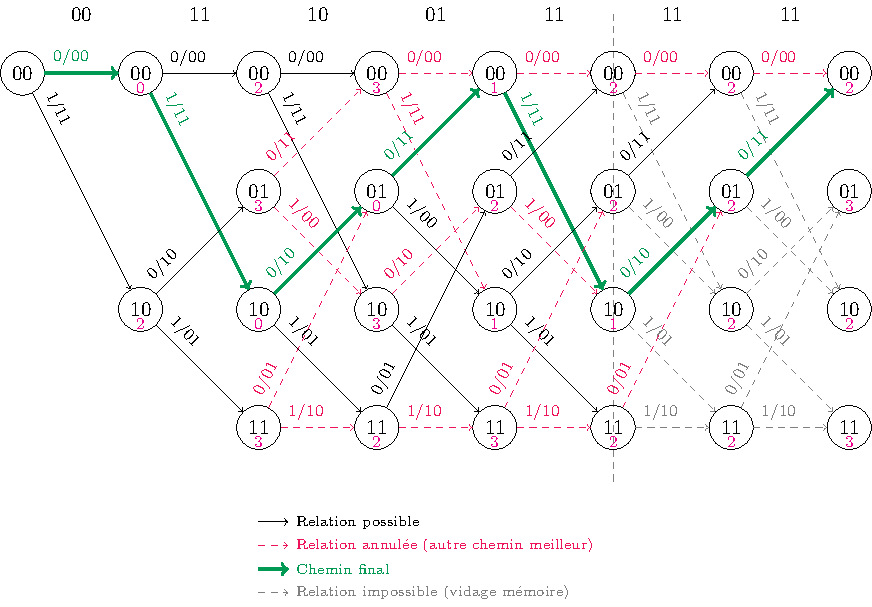
\includegraphics[width=0.9\columnwidth]{Viterbi.pdf}
\end{figure}
Le code corrigé est donc
00 11 10 \textcolor{OrangeRed}{1}1 11 1\textcolor{OrangeRed}{0} 11. Qui correspond à la séquence 0100100 (le message est \textcolor{RoyalBlue}{01001}, les deux derniers bits sont le vidage de la mémoire).
\end{document}